For a set of preliminary experiments, we first focus on SVMs applied
to the grasp type classification problem. The simplest idea is that of
checking whether data obtained during one session can be used to build
a model able to generalise over other sessions during the same
day. Such a result would indeed mean that less than three minutes of
data gathering are potentially able to control the prosthesis for a
long time --- at least one day, if not more.

\begin{figure}[!ht] \centering
  \begin{tabular}{c}
    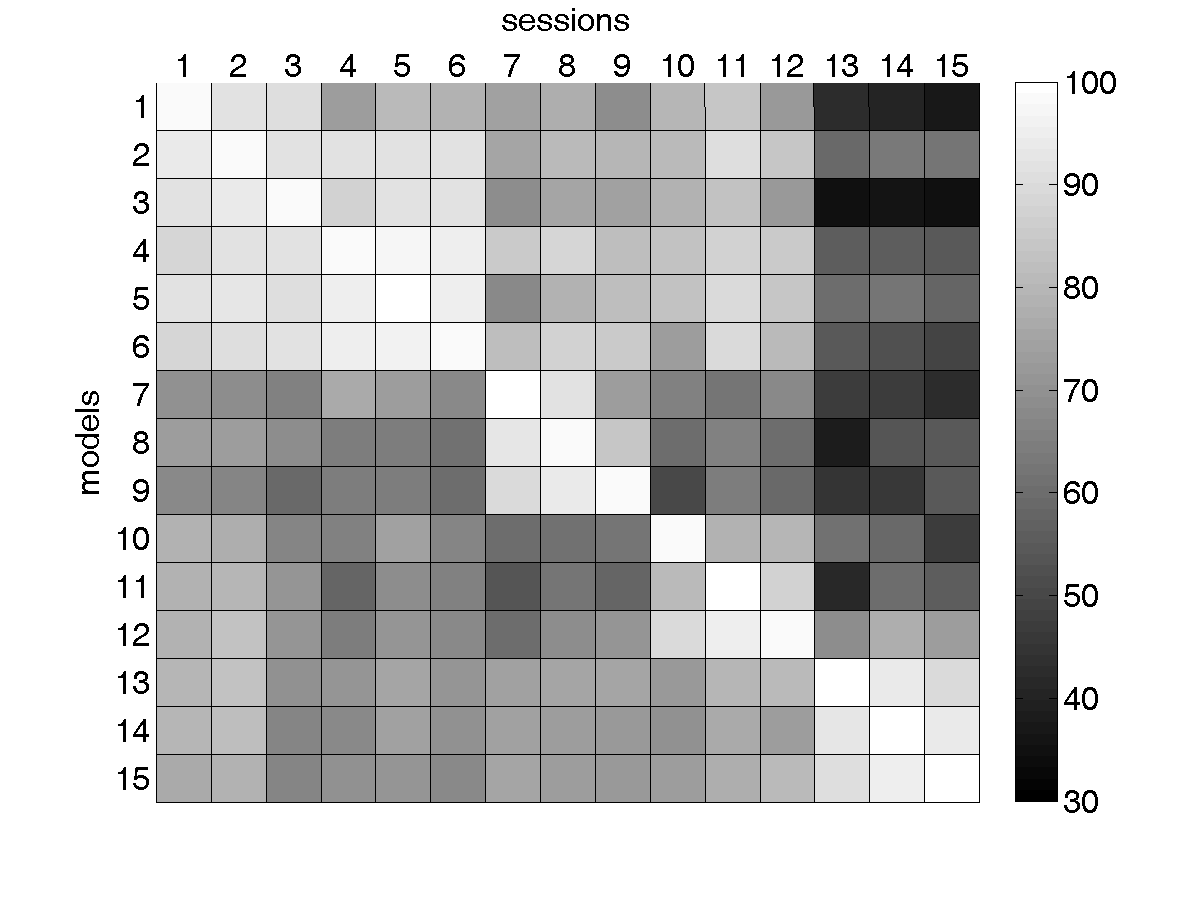
\includegraphics[width=0.45\textwidth]{figs/fig_resCross1_full.png}
  \end{tabular}
  \caption{Accuracy matrix for day $1$. Accuracy for non-diagonal
    elements is $73.23\% \pm 14.29\%$.}
  \label{fig:cross_first}
\end{figure}

In order to check this hypothesis, we trained a SVM for classification
over each single session, for the first day. Sessions are numbered
chronologically during the day, sessions $1,2,3$ forming group $1$,
sessions $4,5,6$ forming group $2$, and so on. (With a slight abuse of
language, we will call the model obtained by training a machine on
session $i$, \emph{model $i$}). We then tested each model on all
sessions of the first day, obtaining therefore an \emph{accuracy
matrix} $A$ in which $A_{ij}$ would be a percentage denoting the
correctly guessed labels when testing model $i$ on session $j$. This
is a \emph{cross-session analysis}. The accuracy matrix $A$ for day
$1$ is visible in Figure \ref{fig:cross_first}.

As one can see, the hypothesis fails: the average accuracy attained on
non-diagonal elements is about $74\%$, dropping down to about $30\%$
in the worst cases (of course, we are not interested in diagonal
elements of the matrix, which represent accuracies obtained by testing
on data on which the models have been trained.). One cannot expect to
correctly drive a prosthesis if one sample in four is
misclassified. Notice that, however, a significant ``group accuracy''
phenomenon is present: in the matrix, good accuracy values are
obtained on $3\times3$ sub-matrices located on the diagonal,
corresponding to cross-session accuracy for sessions \emph{belonging
to the same group}, that is, when the elastic bands were not removed
and no electrode displacement was present. A simple explanation of
this is that electrode displacement shifts the samples in the input
space, causing a decrease in performance. This hypothesis will be used
later on.

Another problem is that there are simply too many samples to train
upon. The total time of data gathering was about $100$ minutes; at
$256$Hz, that means about $1.6$ millions samples, an unfeasibly large
training set for any of the examined methods, not to mention SVM
classification. Even restricting a training set to a single session,
this would result in about $53,000$ samples, which not only is still
too large, but probably contains redundant and irrelevant information.
Moreover, in the real setting, that is on-line, this number is doomed
to grow continually and cannot therefore be used as it is for
periodical re-training. A smart sample reduction strategy is needed,
in order both to overcome this problem, but also to gain insight into
the EMG signal in general.

\subsubsection{Batch Uniformisation}

The simple idea behind batch uniformisation is that, in a real-life
set-up such as ours, there can be many input samples located in the
very same region of the input space, with very similar target
values. One obvious case is that of label $0$, indicating no ongoing
grasping: it is intuitively expected that a large number of samples
will be taken in that region of the input space, since the subject
will be in the $0$ condition for a longer time than all other
labels. 

Since all functions involved in the experiment are due to human
motion, it seems reasonable to assume that they are continuous and
derivable up to any arbitrary order; therefore, it makes little sense
to consider samples obtained in a non-uniform way such as that
described above: if samples are too close to each other (according to
a suitable notion of distance in the input space) than the value of
our target functions should be similar, and non-parametric learning
systems such as SVMs should be able to take it into account.

Batch uniformisation consists of removing, from a training set, those
samples which are \emph{too close to each other}, according to a
suitable notion of inter-sample distance. In order to take into
account the variance of each single electrode, and since in batch data
analysis all data are available beforehand and therefore all possible
statistics can be gathered a-priori, we have decided to adopt
Mahalanobis's distance as the inter-sample distance. Let $\xx_1, \xx_2
\in \RR^{10}$; then the Mahalanobis distance between $\xx_1$ and
$\xx_2$ is defined as

$$ MD(\xx_1,\xx_2) = \sqrt{(\xx_1-\xx_2)^T \Sigma^{-1} (\xx_1-\xx_2)} $$

\noindent where $\Sigma$ is the $10\times10$ covariance matrix, evaluated
on the training set. $MD(\xx_1,\xx_2)$ is a measure of distance
independent of the (co)variance of the electrodes. (Notice that if
$\Sigma$ is replaced by the identity matrix, $MD(\xx_1,\xx_2)$ is
reduced to the usual notion of Euclidean distance.)

Since checking the inter-sample distance on a batch of samples
obviously takes a quadratic time with respect to the number of
samples, which was infeasible, we adopt an approximated method which
removes most, but not necessarily all, samples which are too
Mahalanobis-close to each other. After a few initial experiments, the
threshold distance was set at $1$. Obviously, no \emph{testing} set is
uniformised. Notice, further, that applying uniformisation results in
training sets which are considerably smaller than the original ones,
up to about $100$ times smaller, in fact dramatically decreasing the
time required to train and test.

Consider now Figure \ref{fig:cross_initial}. The Figure presents more
cross-session accuracy analysis, but this time both for the first and
second day, and both with full and uniformised training sets. (If the
training set of a model has been uniformised, we will call the model
\emph{uniform}.)

\begin{figure}[!ht] \centering
  \begin{tabular}{cc}
    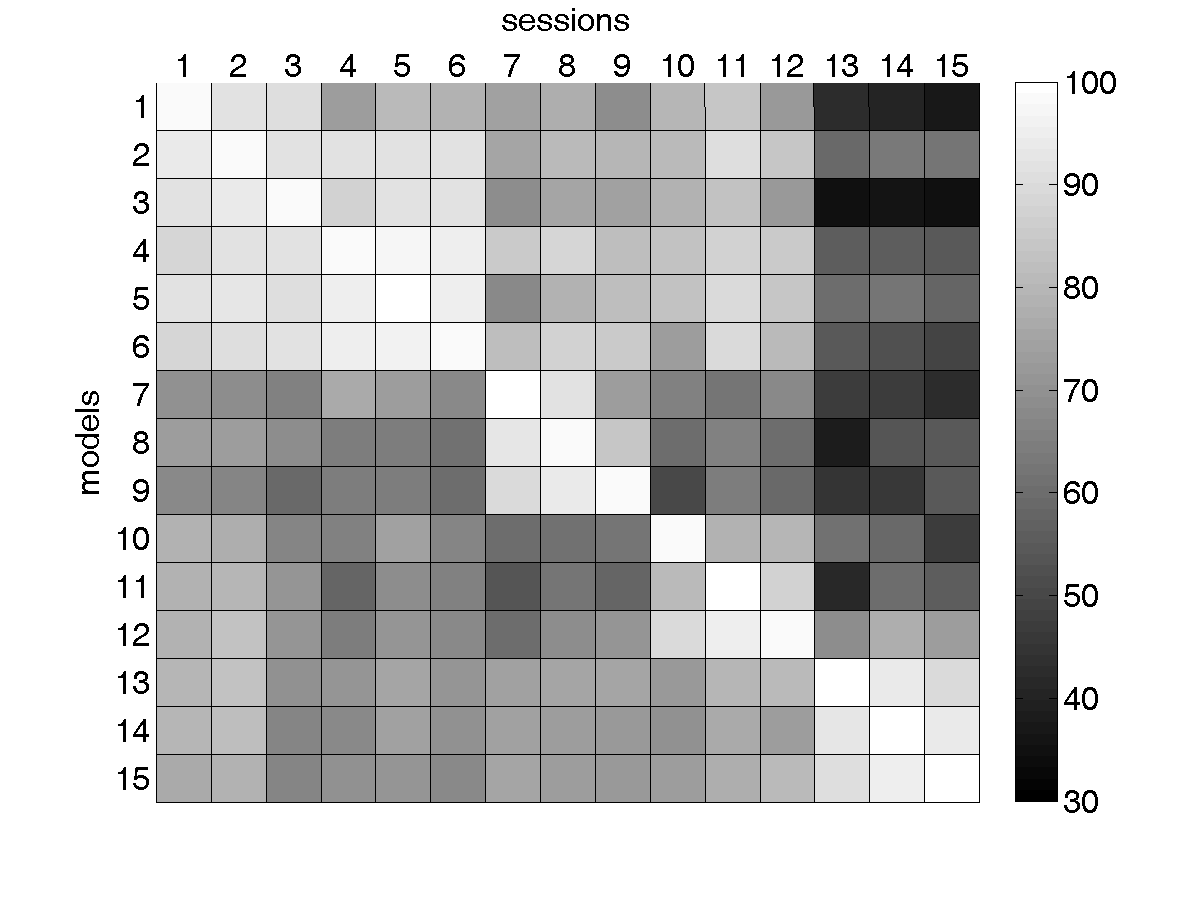
\includegraphics[width=0.23\textwidth]{figs/fig_resCross1_full.png} &
    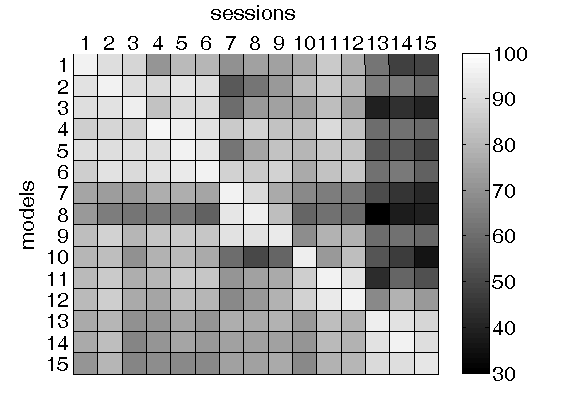
\includegraphics[width=0.23\textwidth]{figs/fig_resCross1.png} \\
    diagonal: $98.73\% \pm 0.39\%$  & diagonal: $95.52\% \pm 1.21\%$ \\
        rest: $73.23\% \pm 14.29\%$ & rest: $74.53\% \pm 13.70\%$ \\
    (a) & (b) \\[5mm]
    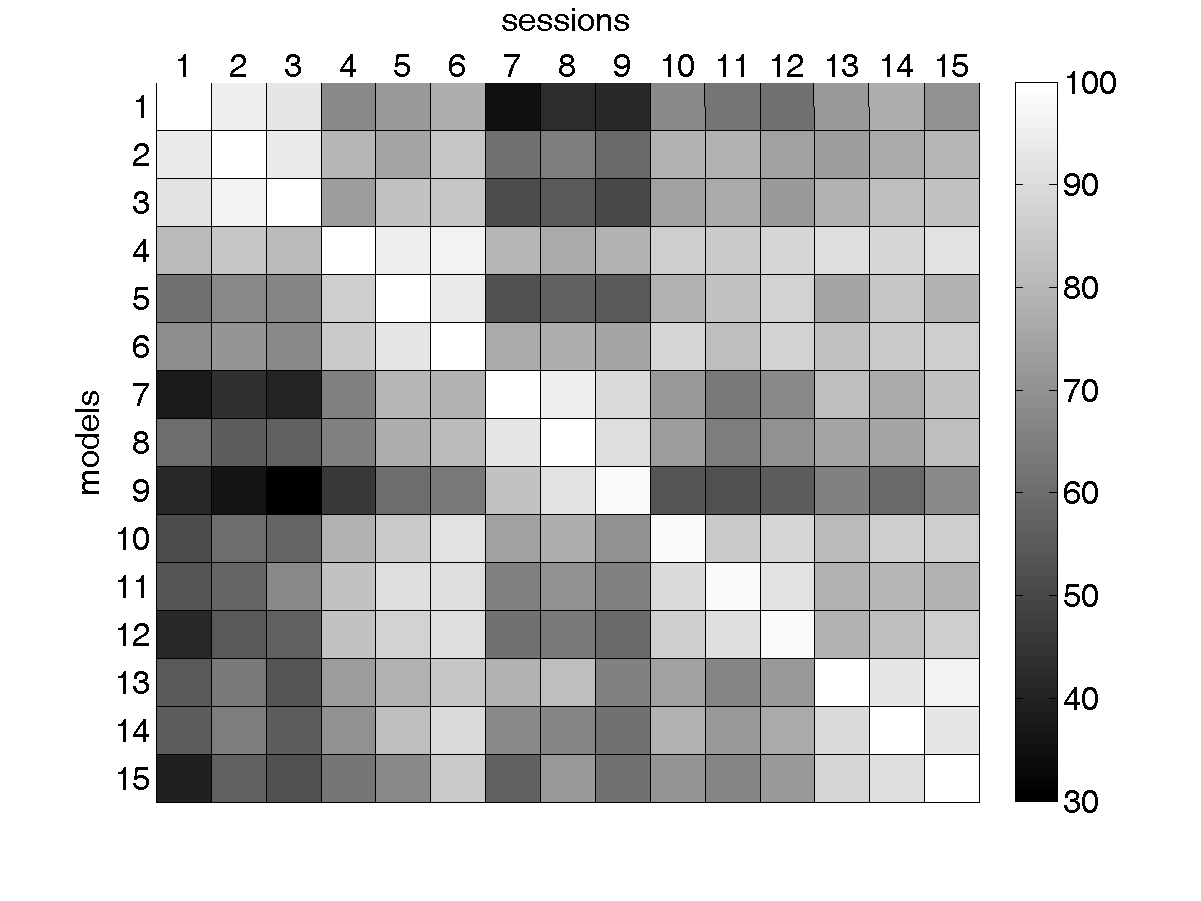
\includegraphics[width=0.23\textwidth]{figs/fig_resCross2_full.png} &
    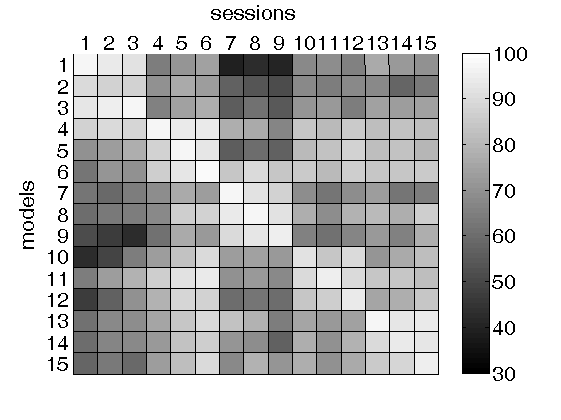
\includegraphics[width=0.23\textwidth]{figs/fig_resCross2.png} \\
    diagonal: $99.05\% \pm 0.37\%$ & diagonal: $95.37\% \pm 2.85\%$ \\
        rest: $73.23\% \pm 14.47\%$ & rest: $74.38\% \pm 12.27\%$ \\
    (c) & (d) \\
  \end{tabular}
  \caption{Cross-session analysis and evaluation of the batch uniformisation
    procedure. $(a)$ and $(b)$, accuracy matrices for day $1$: $(a)$
    full models, $(b)$ uniform models. $(c)$ and $(d)$, same for day $2$.}
  \label{fig:cross_initial}
\end{figure}

Consider first panes (a) and (b) of the Figure, pane (a) being the
accuracy matrix for full models, day $1$, and pane (b) being the
accuracy matrix for the same day, but using uniform models. (Actually,
pane (a) is the same matrix seen in Figure \ref{fig:cross_first}). It
is apparent that uniform models attain a slightly better accuracy on
non-diagonal elements, if compared to the full models. In fact, the
accuracies are $73.23\% \pm 14.29\%$ for the full models, and $74.53\%
\pm 13.70\%$ for the uniform ones. The same analysis for day $2$
yields analogous results (consider the same Figure, panes (c) and
(d)).

From this we conclude that the uniformisation procedure greatly
reduces the training set size (and training and testing times) without
degrading the performance. This is apparent from the fact that uniform
models are slightly more accurate on testing sets which are disjoint
from the training sets. Uniform models generalise slightly better, at
least in this case.

\subsubsection{Classification}

Let us go more in detail, as far as the first day is concerned (Figure
\ref{fig:cross_initial} again, pane (b)): one can see that the first
six models (trained on the first two groups) obtain a quite good
accuracy on the first six sessions (first two groups) whereas their
accuracy rapidly degrades as more sessions are tested for. This is
probably due to the first two groups having been gathered in similar
conditions, very similar electrode positions and/or similar movements
performed by the subject. On the other hand, sessions in the last
group (columns $13$, $14$ and $15$ of the matrix) are particularly
hard, except when tested by models obtained from the last group itself
--- here the effect is probably motivated by the opposite reason:
during those sessions, the subject must have explored different parts
of the input space. This is corroborated by the fact that models
$13,14,15$ perform rather well on \emph{all} sessions, if compared to
other models (check rows $13,14,15$ of the matrix). In other words,
sessions $13,14,15$ contain more relevant information than the others.
Analogous considerations can be made by inspecting the accuracy matrix
of the second day, pane (d) of the Figure.

From this analysis we confirm (recall the previous Subsection) that
\emph{electrode displacement plays a determinant role} in the
classification accuracy. Notice that muscle fatigue seems not to enter
the picture, but this is reasonable since it is present already within
one single session and the machine correctly takes it into account
during the training phase. Notice once again that the uniformisation
procedure does not hinder the generalisation power of the
system. Electrode displacement present between groups (but not within
a group) causes the samples in a group to be ``shifted'' in the input
space, so that testing on a different group results in poor
performance.

If this claim is correct, then there should be (negative) correlation
between distance and accuracy. In fact, cross-session accuracy is
highly correlated to the \emph{average minimum inter-sample distance}
between sessions. More in detail, let $S_i$ and $S_j$ denote the sets
of samples gathered during sessions $i$ and $j$; then the
\emph{cross-session distance matrix} $D$ is such that

$$ D_{ij} = \frac{1}{|S_j|} \sum_{s_j \in S_j}{\min_{s_i \in S_i}{ ||s_j-s_i||^2 } } $$

Essentially, $D_{ij}$ denotes how far away in the input space the
samples in $S_j$ are from the samples in $S_i$. Note that $D$ is in
general not symmetric. The cross-correlation coefficient evaluated
between $D$ and the cross-session accuracy matrix is about $-0.61$
\emph{both} for the first and the second day, indicating a strong
negative correlation. Further experiments have revealed that this
happens for Neural Networks too (cross-correlation $-0.40$ for day $1$
and $-0.51$ for day $2$); and also, that $D$ is strongly
\emph{positively} correlated to the MSE in regression, for all the
studied approaches: $0.62/0.78$ (day $1$/day $2$) for SVMs,
$0.64/0.72$ for FFNs and $0.77/0.81$ for LWPR. In other words, the
larger the distance of $S_i$ and $S_j$, the worse the performance of
model $i$ tested on session $j$, \emph{both in classification and in
regression}, and \emph{for all approaches tested}.

This tells us that (a) samples of the same group are closer to each
other than sample from different groups, therefore electrode
displacement causes displacement in the input space too; and (b) that
this causes bad inter-group performance. ``Samples far away from the
training set will be predicted badly.''

The dual consideration is that if we train upon the ``right'' data,
the accuracy should become acceptable. How to find the right data
then? In this batch phase, we have decided to adjoin two models per
day, which would obtain a good accuracy on all sessions. For instance,
consider Figure \ref{fig:cross_initial} again, pane (b). It is
apparent that model $4$ performs well on groups $1$ to $4$, whereas
model $13$ does well on group $5$ (and is not bad on the
others). These two models were used to form a ``best'' training set
which would give good results on the whole day $1$. Analogous
considerations led us to use also models $4$ and $8$ of day $2$. The
obtained model will be called \emph{best} model.

This procedure was repeated for each problem tackled (classification,
regression) and approach tested (SVM, FFN, and LWPR). Figure
\ref{fig:best_class} shows the classification accuracy of the best
models for classification on all sessions of day $1$ and $2$, for SVMs
and FFNs. The analysis detailed in the previous Subsection has been
repeated for the Neural Network. In that case, models $8$ and $15$ of
day $1$, and models $3$ and $10$ of day $2$ have been used to build
the best model.

\begin{figure}[!ht] \centering
  \begin{tabular}{cc}
    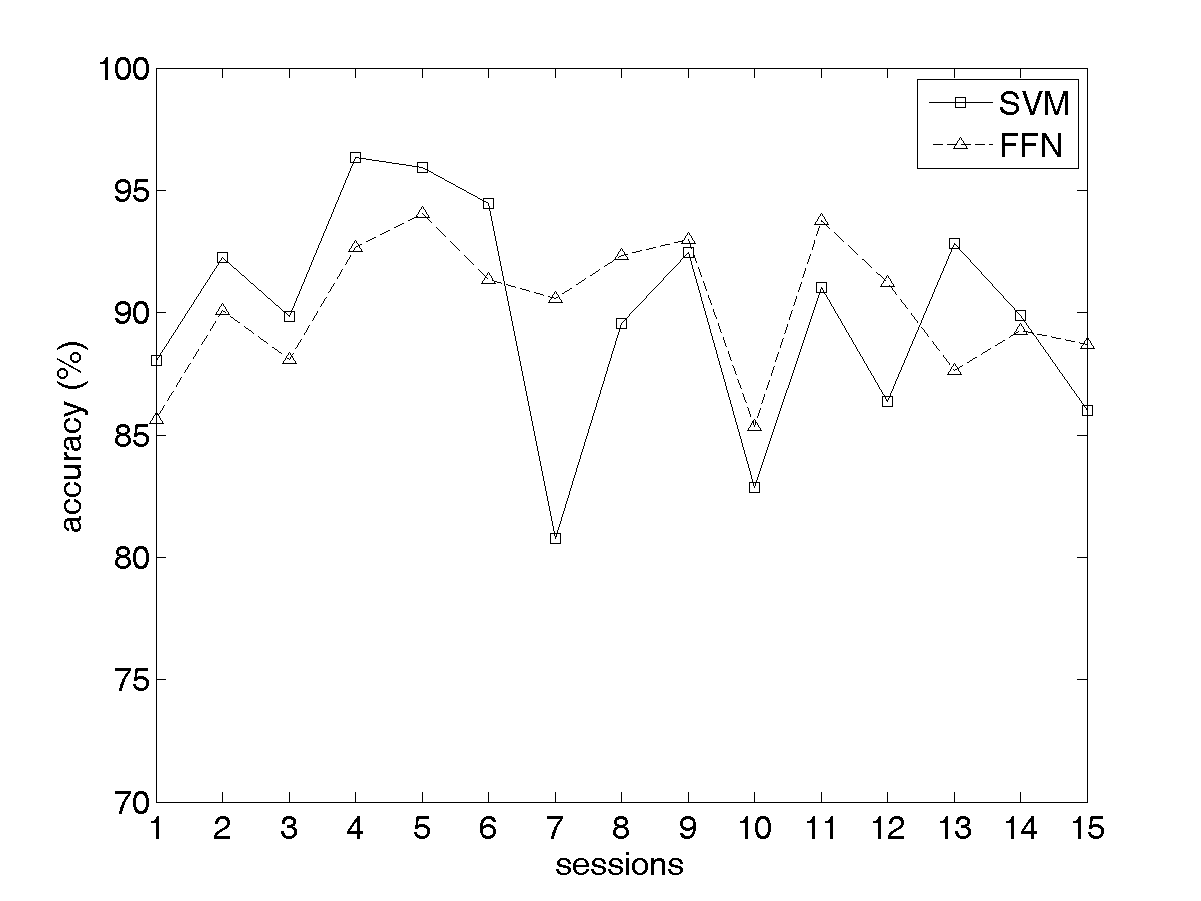
\includegraphics[width=0.23\textwidth]{figs/fig_class_resCrossBestOnDay1.png} &
    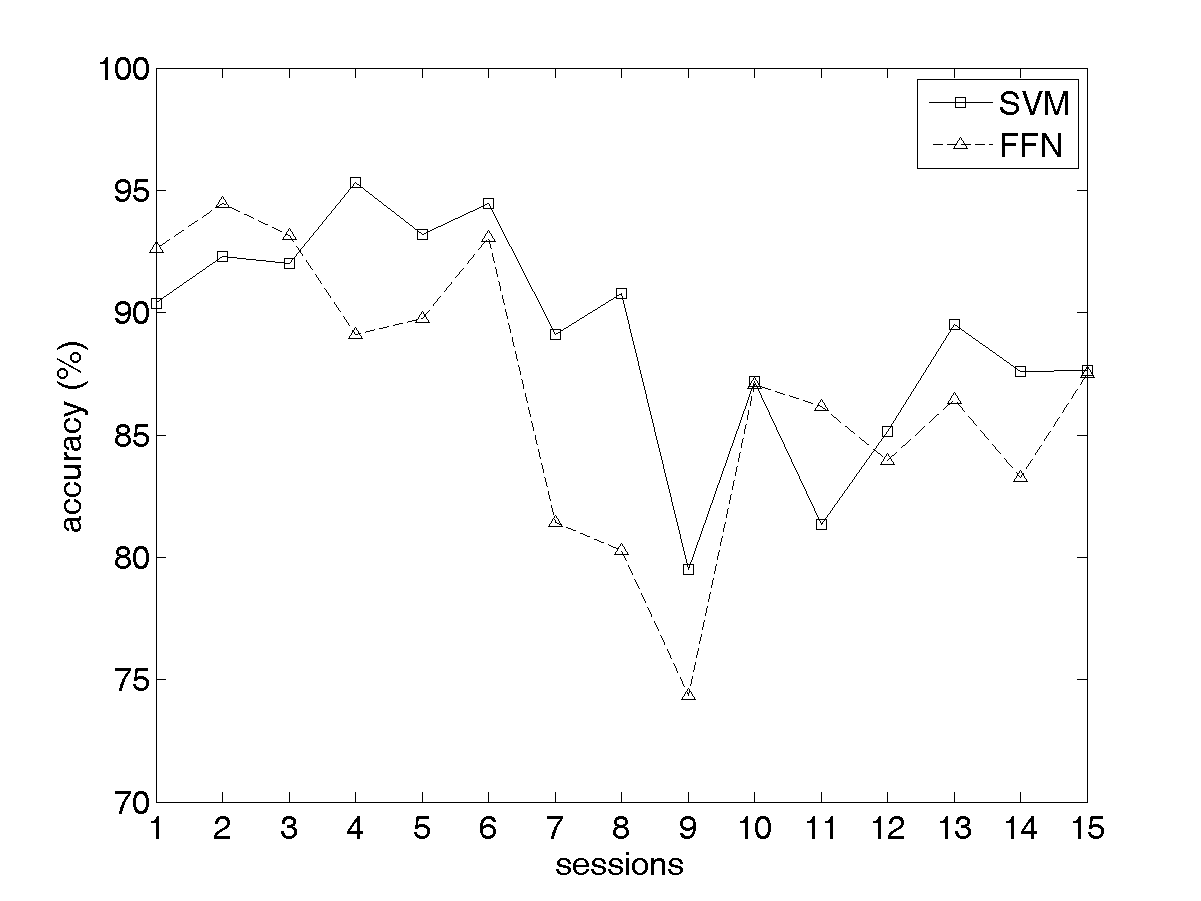
\includegraphics[width=0.23\textwidth]{figs/fig_class_resCrossBestOnDay2.png} \\
    SVM: $89.90\% \pm 4.51\%$ & SVM: $89.04\% \pm 4.50\%$ \\
    FFN: $90.25\% \pm 2.77\%$ & FFN: $86.84\% \pm 5.57\%$ \\
    $(a)$ & $(b)$ \\
  \end{tabular}
  \caption{Classification accuracy of best models, day $1$ $(a)$ and
    day $2$ $(b)$.}
  \label{fig:best_class}
\end{figure}

As one can see, there is no clear winner between SVMs and FFNs. FFNs
perform slightly better on day $1$ (higher mean, lower standard
deviation) but SVMs are analogously better on day $2$. All in all,
classification accuracy is good, at an overall rate of about
$90\%$. In this case, the training data amounts to four sessions
(uniformised in the case of SVMs and full in the case of FFNs), which
is about $12$--$15$ minutes of user activity. But notice, that samples
gathered during both days were necessary to have an idea of which
sessions to use.

\subsubsection{Regression}

Lastly, the most interesting part was how to predict the amount of
force applied by the subject by looking at the EMG signal. To do this,
we have repeated once again the analysis done in Subsection
\ref{subsec:strategy} for the three approaches selected, and found out
that the four sessions involved in the best models were: $6,12,3,12$
for SVMs, $4,11,3,12$ for FFNs and $6,13,3,4$ for LWPR. We have
considered three indices of performance: the Mean Squared Error (MSE)
in its standard definition; the Normalised Root MSE (NRMSE), ratio of
the square root of the MSE and the range of the target values,
expressed as a percentage; and the Squared Correlation Coefficient
(SCC) between the predicted target and the real target.

\begin{figure}[!ht] \centering
  \begin{tabular}{cc}
    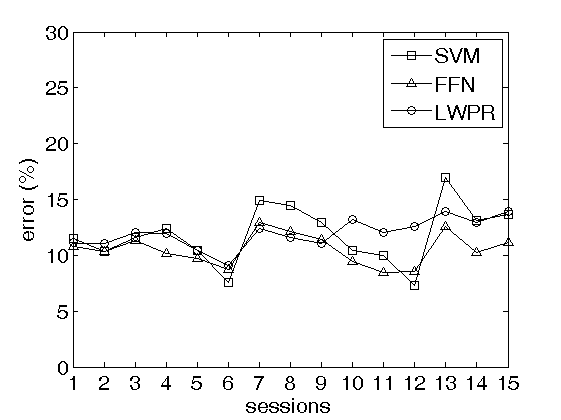
\includegraphics[width=0.23\textwidth]{figs/fig_err_regr_resCrossBestOnDay1.png} &
    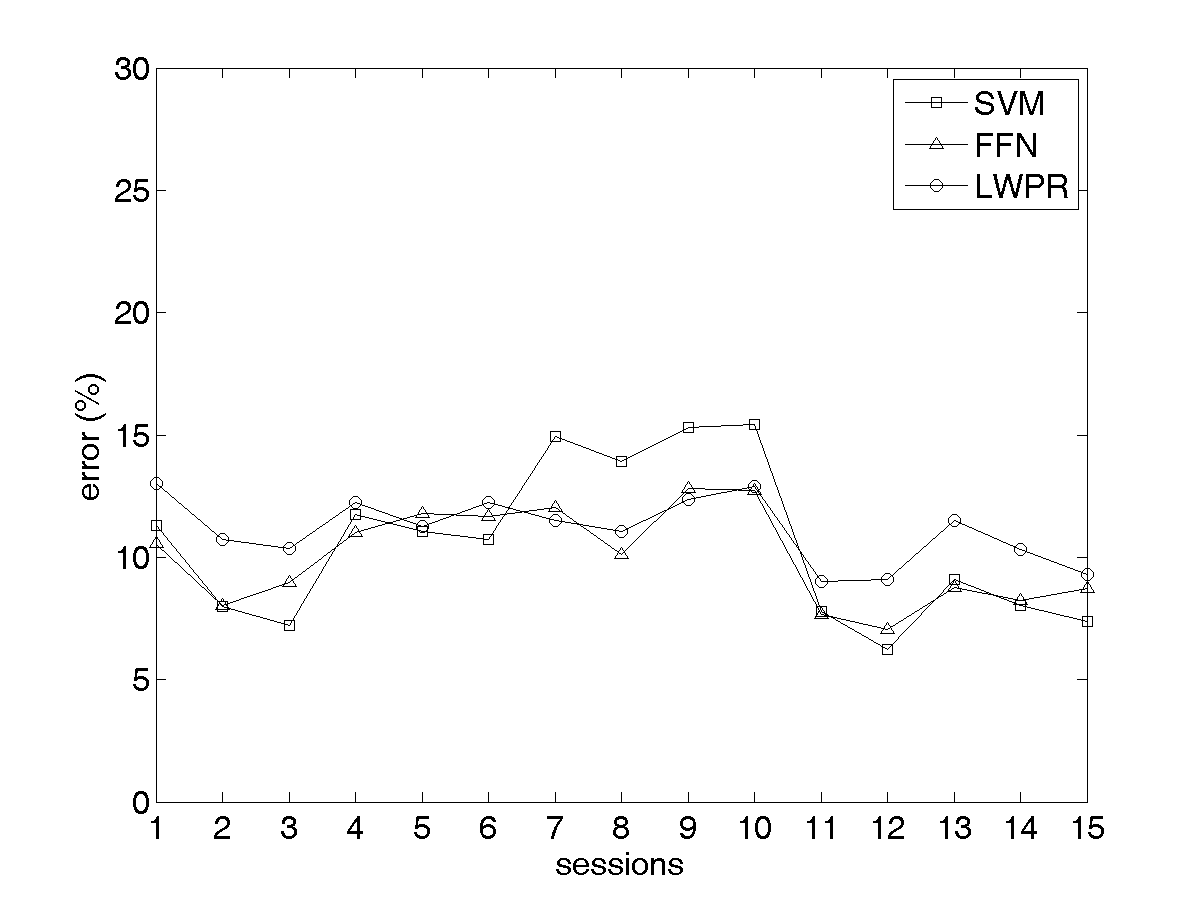
\includegraphics[width=0.23\textwidth]{figs/fig_err_regr_resCrossBestOnDay2.png} \\
     SVM: $11.84\% \pm 2.64\%$ &  SVM: $10.54\% \pm 3.18\%$ \\
     FFN: $10.54\% \pm 1.41\%$ &  FFN: $10.01\% \pm 1.93\%$ \\
    LWPR: $11.98\% \pm 1.31\%$ & LWPR: $11.13\% \pm 1.32\%$ \\
    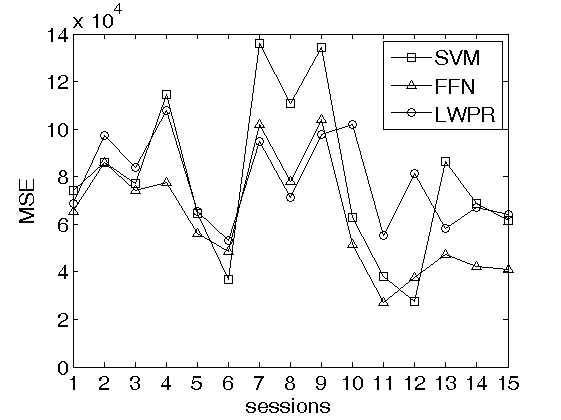
\includegraphics[width=0.23\textwidth]{figs/fig_MSE_regr_resCrossBestOnDay1.png} &
    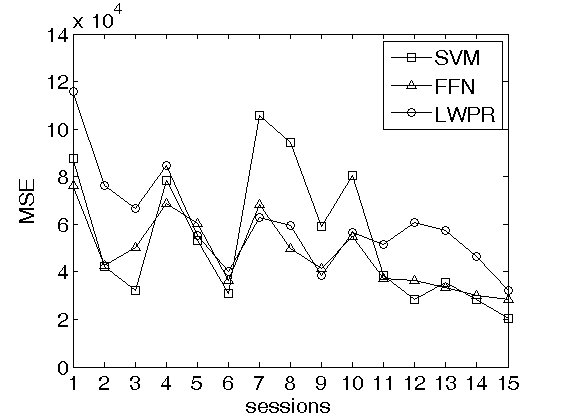
\includegraphics[width=0.23\textwidth]{figs/fig_MSE_regr_resCrossBestOnDay2.png} \\
     SVM: $7.86 \pm 3.35$ &  SVM: $5.44 \pm 2.79$ \\
     FFN: $6.27 \pm 2.36$ &  FFN: $4.76 \pm 1.52$ \\
    LWPR: $7.79 \pm 1.83$ & LWPR: $6.03 \pm 2.07$ \\
    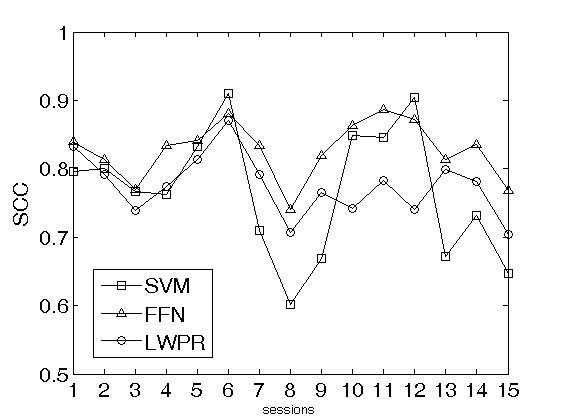
\includegraphics[width=0.23\textwidth]{figs/fig_SCC_regr_resCrossBestOnDay1.png} &
    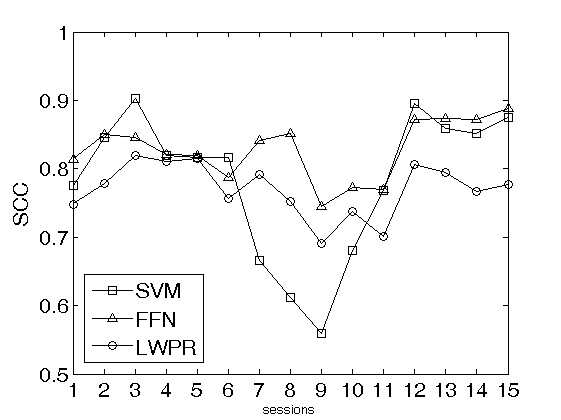
\includegraphics[width=0.23\textwidth]{figs/fig_SCC_regr_resCrossBestOnDay2.png} \\
     SVM: $0.77 \pm 0.09$ &  SVM: $0.78 \pm 0.11$ \\
     FFN: $0.83 \pm 0.04$ &  FFN: $0.83 \pm 0.04$ \\
    LWPR: $0.78 \pm 0.05$ & LWPR: $0.77 \pm 0.04$ \\
  \end{tabular}
  \caption{Regression accuracy of best models, day $1$ (left panes)
    and day $2$ (right panes). First row: Normalised Root MSE; second
    row: Mean Squared Error; third row, Squared Correlation Coefficient.}
  \label{fig:best_regr}
\end{figure}

Figure \ref{fig:best_regr} shows the results; left panes are for day
$1$ and right panes for day $2$. Consider the first row, plotting the
NRMSE for each session: as it is apparent, as it was for
classification, there is no clear advantage of one approach over
another. FFNs perform slightly better as far as the NRMSE is concerned,
which is probably the most interesting measure of performance, when
moving to a real setting. Their error is on average $10.54\% \pm
1.41\%$ and $10.01\% \pm 1.93\%$. But as well, both LWPR and SVM
perform quite well, their average errors ranging from $10.54\%$ to
$11.98\%$.

Consider now the second and third rows of the Figure. First of all
there is a clear inverse correlation between the MSE and the SCC, as
expected. Secondly, it is once again clear that the generalisation
performance strongly depends on which data we have used to train the
machines: consider for instance the MSE attained by SVM on day $1$
(Figure \ref{fig:best_regr}, second row, left pane, blue curve): the
best model was trained upon data coming from sessions $6$ and $12$,
although uniformised, and not surprisingly those are the sessions for
which the MSE is minimum; the same effect is present for the other
approaches.

Lastly, in practical terms: the best average MSE obtained by FFNs
($6.27\cdot 10^4 \pm 2.36\cdot 10^4$ and $4.76\cdot 10^4 \pm 1.52\cdot
10^4$) corresponds to, in turn, an average error of 5N and
4.36N. Figure \ref{fig:regression} shows some samples of the force
values obtained from the OFTS, along with the corresponding values
predicted by the best approach, that is, FFNs. As one can see, despite
the non perfect correspondence of the two curves, the FFN definitely
follows the real target to a remarkable degree of accuracy, for a wide
range of frequencies of the pressing/releasing action. The Figure
shows data taken from three different sessions, in decreasing order of
performance.

\begin{figure*}[!ht] \centering
  \begin{tabular}{ccc}
    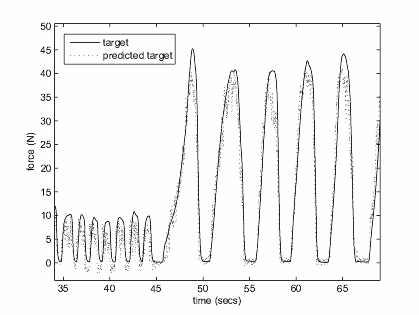
\includegraphics[width=0.30\textwidth]{figs/fig_regression1.png} &
    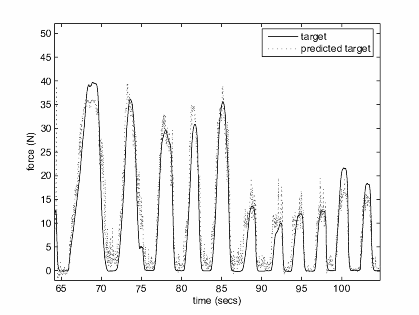
\includegraphics[width=0.30\textwidth]{figs/fig_regression2.png} &
    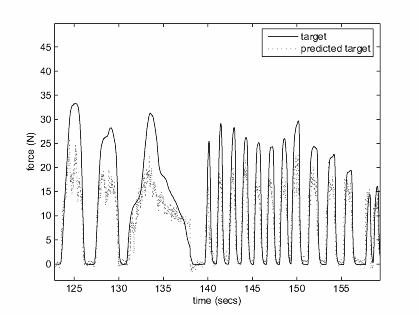
\includegraphics[width=0.30\textwidth]{figs/fig_regression3.png} \\
    session $6$, day $1$ & session $10$, day $2$ & session $7$, day $1$ \\
    MSE: $4.85\cdot 10^4$ & MSE: $5.48\cdot 10^4$ & MSE: $10.21\cdot 10^4$ \\
  \end{tabular}
  \caption{Examples of real and predicted force target values.}
  \label{fig:regression}
\end{figure*}

A remarkable point in the Figure is the presence of a ``plateau''
effect, especially in the test with the worst performance, namely
session $7$ of day $1$ (third pane). As is apparent, the predicted
target are mostly wrong in amplitude, being systematically
\emph{lower} than the correct values. Again, this is most likely due
to insufficient sampling in the region of interest.
